%%%%%%%%%%%%%%%%%%%%%%%%%%%%%%%%%%%%%%%%%%%%%%%%%%%%%%%%%%%%%%%%%%%%%%
% Template de Artigo
% XXIX ENMC – Encontro Nacional de Modelagem Computacional
% XVII ECTM – Encontro de Ciência e Tecnologia de Materiais
%%%%%%%%%%%%%%%%%%%%%%%%%%%%%%%%%%%%%%%%%%%%%%%%%%%%%%%%%%%%%%%%%%%%%%

\documentclass[12pt,fleqn]{article}

%%%%%%%%%%%%%%%%%%%%%%%%%%%%%%%%%%%%%%%%%%%%%%%%%%%%%%%%%%%%%%%%%%%%%%
% CONFIGURAÇÃO DE IDIOMA E CODIFICAÇÃO
%%%%%%%%%%%%%%%%%%%%%%%%%%%%%%%%%%%%%%%%%%%%%%%%%%%%%%%%%%%%%%%%%%%%%%

\usepackage[utf8]{inputenc}
\usepackage[T1]{fontenc}
\usepackage[brazil]{babel}

%%%%%%%%%%%%%%%%%%%%%%%%%%%%%%%%%%%%%%%%%%%%%%%%%%%%%%%%%%%%%%%%%%%%%%
% PACOTES DO TEMPLATE
%%%%%%%%%%%%%%%%%%%%%%%%%%%%%%%%%%%%%%%%%%%%%%%%%%%%%%%%%%%%%%%%%%%%%%

\usepackage{setup/config}
\usepackage{natbib}
\usepackage{graphicx}
\usepackage{color}
\usepackage{wallpaper}
\usepackage{hyperref}
\usepackage{titlesec}
\usepackage{float}
\usepackage{fancyhdr}
\usepackage{booktabs}
\usepackage{siunitx}
\setlength{\headheight}{20.68497pt}
\addtolength{\topmargin}{-8.68497pt}

%%%%%%%%%%%%%%%%%%%%%%%%%%%%%%%%%%%%%%%%%%%%%%%%%%%%%%%%%%%%%%%%%%%%%%
% DIRETÓRIO DAS FIGURAS
%%%%%%%%%%%%%%%%%%%%%%%%%%%%%%%%%%%%%%%%%%%%%%%%%%%%%%%%%%%%%%%%%%%%%%

\graphicspath{{figures/}}

%%%%%%%%%%%%%%%%%%%%%%%%%%%%%%%%%%%%%%%%%%%%%%%%%%%%%%%%%%%%%%%%%%%%%%
% AJUSTE DE ESPAÇAMENTO NA BIBLIOGRAFIA
%%%%%%%%%%%%%%%%%%%%%%%%%%%%%%%%%%%%%%%%%%%%%%%%%%%%%%%%%%%%%%%%%%%%%%

\let\OLDthebibliography\thebibliography
\renewcommand\thebibliography[1]{%
\OLDthebibliography{#1}
\setlength{\parskip}{0pt}
\setlength{\itemsep}{0pt plus 0.3ex}
}

%%%%%%%%%%%%%%%%%%%%%%%%%%%%%%%%%%%%%%%%%%%%%%%%%%%%%%%%%%%%%%%%%%%%%%
% TÍTULO DO ARTIGO
%%%%%%%%%%%%%%%%%%%%%%%%%%%%%%%%%%%%%%%%%%%%%%%%%%%%%%%%%%%%%%%%%%%%%%

\title{SISTEMA DE RECUPERAÇÃO AUTO ROTATIVO BIOINSPIRADO (SRAB) PARA NANOSSATÉLITE POCKETQUBE 1P: FUNDAMENTAÇÃO, MODELAGEM, VALIDAÇÃO EXPERIMENTAL PRELIMINAR E SIMULAÇÃO COMPUTACIONAL}

%%%%%%%%%%%%%%%%%%%%%%%%%%%%%%%%%%%%%%%%%%%%%%%%%%%%%%%%%%%%%%%%%%%%%%
% AUTORES E AFILIAÇÕES
%%%%%%%%%%%%%%%%%%%%%%%%%%%%%%%%%%%%%%%%%%%%%%%%%%%%%%%%%%%%%%%%%%%%%%

\author{
\rm
\begin{tabular}{l}
\textbf{Diego dos Santos Alves}$^{1}$ - {\textnormal diego.alves@grad.iprj.uerj.br}\\
\textbf{Pedro Henrique Couto Silva}$^{1}$ - {\textnormal pedro.silva@grad.iprj.uerj.br}\\
\textbf{Vinicius Carvalho Monnerat Bandeira}$^{1}$ - {\textnormal vinicius.bandeira@grad.iprj.uerj.br}\\
\textbf{Pablo Alves Mattos Borges}$^{1}$ - {\textnormal pablo.borges@grad.iprj.uerj.br}\\
\textbf{Angelo Mondaini Calvão}$^{1}$ - {\textnormal oangelo@iprj.uerj.br}\\
\textbf{Eustáquio de Souza Baêta Júnior}$^{2}$ - {\textnormal eustaquio.baeta@eng.uerj.br}\\
\textbf{Letícia dos Santos Aguilera}$^{3}$ - {\textnormal leticia.aguilera@iprj.uerj.br}\\
{\fontsize{11}{0}\selectfont $^{1}$Universidade do Estado do Rio de Janeiro, Instituto Politécnico -- Nova Friburgo -- RJ}\\
{\fontsize{11}{0}\selectfont $^{2}$Universidade do Estado do Rio de Janeiro, Faculdade de Engenharia, Programa de Pós-Graduação em Engenharia Mecânica -- Rio de Janeiro -- RJ}\\
{\fontsize{11}{0}\selectfont $^{3}$Universidade do Estado do Rio de Janeiro, Instituto Politécnico, Programa de Pós-Graduação em Ciência e Tecnologia de Materiais -- Nova Friburgo -- RJ}
\end{tabular}
}

%%%%%%%%%%%%%%%%%%%%%%%%%%%%%%%%%%%%%%%%%%%%%%%%%%%%%%%%%%%%%%%%%%%%%%
% RODAPÉ ESPECIAL DA PRIMEIRA PÁGINA
%%%%%%%%%%%%%%%%%%%%%%%%%%%%%%%%%%%%%%%%%%%%%%%%%%%%%%%%%%%%%%%%%%%%%%

\fancypagestyle{firstpagestyle}
{
\renewcommand{\headrulewidth}{0pt}

\fancyfoot[C]{
\footnotesize
\parbox{15cm}{
\centering
\fontsize{7.5}{0}\selectfont\it
XXIX ENMC -- Encontro Nacional de Modelagem Computacional\\
XVII ECTM -- Encontro de Ciência e Tecnologia de Materiais\\
06 a 09 de outubro de 2026 - Bento Gonçalves - RS
}}
}

%%%%%%%%%%%%%%%%%%%%%%%%%%%%%%%%%%%%%%%%%%%%%%%%%%%%%%%%%%%%%%%%%%%%%%
% INÍCIO DO DOCUMENTO
%%%%%%%%%%%%%%%%%%%%%%%%%%%%%%%%%%%%%%%%%%%%%%%%%%%%%%%%%%%%%%%%%%%%%%

\begin{document}

\pretolerance=10000

%%%%%%%%%%%%%%%%%%%%%%%%%%%%%%%%%%%%%%%%%%%%%%%%%%%%%%%%%%%%%%%%%%%%%%
% LOGO DO EVENTO
%%%%%%%%%%%%%%%%%%%%%%%%%%%%%%%%%%%%%%%%%%%%%%%%%%%%%%%%%%%%%%%%%%%%%%

\begin{figure}
\centering

\includegraphics[width=6.25in]{logo.png}
\end{figure}

\vspace{-3cm}

%%%%%%%%%%%%%%%%%%%%%%%%%%%%%%%%%%%%%%%%%%%%%%%%%%%%%%%%%%%%%%%%%%%%%%
% TÍTULO
%%%%%%%%%%%%%%%%%%%%%%%%%%%%%%%%%%%%%%%%%%%%%%%%%%%%%%%%%%%%%%%%%%%%%%

\maketitle

\pagestyle{empty}
\thispagestyle{firstpagestyle}

%%%%%%%%%%%%%%%%%%%%%%%%%%%%%%%%%%%%%%%%%%%%%%%%%%%%%%%%%%%%%%%%%%%%%%
% RESUMO
%%%%%%%%%%%%%%%%%%%%%%%%%%%%%%%%%%%%%%%%%%%%%%%%%%%%%%%%%%%%%%%%%%%%%%

\begin{abstract}
A recuperação de nanossatélites PocketQube 1P depende tradicionalmente de paraquedas, que apresentam pontos únicos de falha como erros de dobradura, costura ou corrosão. Este trabalho propõe o Sistema de Recuperação Auto Rotativo Bioinspirado (SRAB), baseado no mecanismo de autorrotação passiva observado em sementes de samara (\textit{Acer rubrum}, \textit{Fraxinus}). O sistema utiliza arquitetura estrutural assimétrica que induz rotação cônica sem atuação ativa, gerando um Vórtice de Bordo de Ataque (LEV) que reduz a velocidade terminal. A validação emprega modelo dinâmico de quarta ordem (Newton-Euler reduzido) acoplado à Teoria do Elemento de Pá (BEM), implementado no simulador Samara PQ em Python, e ensaios experimentais de queda livre qualitativos com dois protótipos iterativos (Testes 1 e 2). A simulação computacional da configuração Asa3.DXF com 4 asas (Teste 3 -- Parte A) resultou em velocidade de impacto de 12,90~m/s, conicidade de equilíbrio de 17,22$^\circ$ e spin de 372~RPM. Análise de dispersão por Monte Carlo (200 iterações) indicou velocidade de impacto de 12,89~$\pm$~0,20~m/s (P95~=~13,19~m/s). A instrumentação embarcada (ESP32-C3, ICM-20602, BMP280, LoRa RFM95W) foi validada funcionalmente em 20~Hz.
\end{abstract}

\begin{keywords}
Recuperação passiva, samara, PocketQube, autorrotação, Monte Carlo
\end{keywords}

%%%%%%%%%%%%%%%%%%%%%%%%%%%%%%%%%%%%%%%%%%%%%%%%%%%%%%%%%%%%%%%%%%%%%%
% CABEÇALHO DAS DEMAIS PÁGINAS
%%%%%%%%%%%%%%%%%%%%%%%%%%%%%%%%%%%%%%%%%%%%%%%%%%%%%%%%%%%%%%%%%%%%%%

\fancyhead[L]{\footnotesize{\fontsize{7.5}{0}\selectfont\it
XXIX ENMC, XVII ECTM\\
06 a 09 de outubro de 2026}}

\renewcommand{\headrulewidth}{0pt}

\fancyfoot[C]{
\footnotesize
\parbox{15cm}{
\centering
\fontsize{7.5}{0}\selectfont\it
XXIX ENMC -- Encontro Nacional de Modelagem Computacional\\
XVII ECTM -- Encontro de Ciência e Tecnologia de Materiais\\
06 a 09 de outubro de 2026 - Bento Gonçalves - RS
}}

\rhead{}

\pagestyle{fancy}

%%%%%%%%%%%%%%%%%%%%%%%%%%%%%%%%%%%%%%%%%%%%%%%%%%%%%%%%%%%%%%%%%%%%%%
% 1. INTRODUÇÃO
%%%%%%%%%%%%%%%%%%%%%%%%%%%%%%%%%%%%%%%%%%%%%%%%%%%%%%%%%%%%%%%%%%%%%%

\section{INTRODUÇÃO}

O regulamento da Latin American Space Challenge (LASC) exige que sistemas de recuperação de nanossatélites assegurem descida controlada entre 20~m/s e 45~m/s \citep{lasc2026}. Paraquedas, embora difundidos, apresentam pontos únicos de falha em dobraduras, costuras e mecanismos de acionamento. Como alternativa, propõe-se o Sistema de Recuperação Auto Rotativo Bioinspirado (SRAB), de arquitetura passiva inspirada na autorrotação de sementes de samara (\textit{Acer rubrum}, \textit{Fraxinus}). A assimetria estrutural induz rotação cônica estável, gerando Vórtices de Bordo de Ataque (LEV) que ampliam a sustentação efetiva \citep{lentink2009, mcconnell2023} sem atuadores ou lógicas de disparo.

Os objetivos específicos deste trabalho são: (a) desenvolver e validar qualitativamente o modelo dinâmico de 4$^{\underline{a}}$ ordem do SRAB por meio de ensaios de queda livre com protótipos iterativos (Testes 1 e 2); (b) projetar e validar funcionalmente a instrumentação embarcada para aquisição de dados de voo a 20~Hz (Teste 3 -- Parte B); (c) realizar simulação computacional da configuração Asa3 com 4 asas em altitude operacional para caracterizar o regime estacionário e analisar a dispersão paramétrica via Monte Carlo (Teste 3 -- Parte A); (d) realizar análise de sensibilidade paramétrica para caracterizar a influência dos coeficientes aerodinâmicos no regime estacionário; (e) comparar o desempenho do SRAB com sistema de paraquedas equivalente.

O escopo delimita-se à validação preliminar qualitativa (Testes 1 e 2), à análise de sensibilidade paramétrica, à validação funcional da instrumentação e à demonstração de viabilidade física. Não se pretende esgotar a caracterização quantitativa do regime terminal, mas estabelecer bases para investigações futuras, incluindo lançamento real em altitude operacional.

%%%%%%%%%%%%%%%%%%%%%%%%%%%%%%%%%%%%%%%%%%%%%%%%%%%%%%%%%%%%%%%%%%%%%%
% 2. PLATAFORMA FÍSICA
%%%%%%%%%%%%%%%%%%%%%%%%%%%%%%%%%%%%%%%%%%%%%%%%%%%%%%%%%%%%%%%%%%%%%%

\section{PLATAFORMA FÍSICA -- FRAME POCKETQUBE 1P}

A plataforma PocketQube 1P utilizada foi doada à equipe Serra Rocketry durante a edição de 2025 da LASC por um representante da Alba Orbital. A estrutura é composta por frame de alumínio (50~$\times$~50~$\times$~50~mm) e backplate de FR4, com massa total de 44~g. O padrão 1P define massa máxima de 250~g, deixando margem de 206~g para subsistemas de recuperação, eletrônica embarcada e asas.

%%%%%%%%%%%%%%%%%%%%%%%%%%%%%%%%%%%%%%%%%%%%%%%%%%%%%%%%%%%%%%%%%%%%%%
% 3. FUNDAMENTAÇÃO BIOLÓGICA
%%%%%%%%%%%%%%%%%%%%%%%%%%%%%%%%%%%%%%%%%%%%%%%%%%%%%%%%%%%%%%%%%%%%%%

\section{FUNDAMENTAÇÃO BIOLÓGICA}

Sementes de \textit{Acer rubrum} e \textit{Fraxinus} desenvolveram mecanismo de dispersão baseado em autorrotação passiva. A assimetria estrutural, massa concentrada na semente e superfície aerodinâmica expandida na asa, induz rotação cônica estável, reduzindo a velocidade terminal e maximizando a distância de dispersão horizontal \citep{limacher2015, european2009}. Durante a rotação, forma-se um vórtice no bordo de ataque (Leading-Edge Vortex, LEV) que reduz a pressão no extradorso, elevando a sustentação efetiva \citep{lentink2009, mcconnell2023}. \cite{lentink2009} demonstraram que sementes autorrotativas geram LEV estável, mecanismo convergente com o voo de insetos, reproduzível em laboratório \citep{rezgui2020}.

%%%%%%%%%%%%%%%%%%%%%%%%%%%%%%%%%%%%%%%%%%%%%%%%%%%%%%%%%%%%%%%%%%%%%%
% 4. METODOLOGIA
%%%%%%%%%%%%%%%%%%%%%%%%%%%%%%%%%%%%%%%%%%%%%%%%%%%%%%%%%%%%%%%%%%%%%%

\section{METODOLOGIA}

\subsection{Modelagem dinâmica e aerodinâmica}

Construiu-se modelo dinâmico de 4$^{\underline{a}}$ ordem fundamentado nas equações reduzidas de Newton-Euler, com simplificações: ângulo de rolagem lateral desprezível ($\psi \approx 0$), momento de inércia longitudinal nulo ($I_{x3x3}=0$) e inércia em guinada equivalente à de arfagem ($I_{z3z3}=I_{y3y3}$). O vetor de estado é definido por quatro variáveis: ângulo de conicidade ($\theta$), taxa de arfagem ($\dot\theta$), taxa de rotação ($\dot\phi$) e velocidade vertical ($v_0$):

\begin{equation}
\frac{d\theta}{dt} = \dot\theta
\end{equation}

\begin{equation}
\ddot\theta = -\frac{M_{y3}}{I_{y3y3}} - \dot\phi^2 \sin\theta \cos\theta
\end{equation}

\begin{equation}
\ddot\phi = \frac{M_{z3}}{I_{y3y3} \cos\theta} + 2\,\dot\phi\,\dot\theta \tan\theta
\end{equation}

\begin{equation}
\dot v_0 = -g + \frac{F_{z3} \cos\theta}{m}
\end{equation}

As forças aerodinâmicas ($F_{z3}$) e momentos ($M_{y3}$, $M_{z3}$) foram calculados pela Teoria do Elemento de Pá (BEM) com integração numérica ao longo da extensão da asa. Incorporou-se fator de sintonia fenomenológica ($C_{D0}$) para capturar o ganho de sustentação induzido pelo LEV, calibrado iterativamente contra observações experimentais.

\subsection{Simulação computacional (Pipeline Samara PQ)}

O simulador Samara PQ, desenvolvido em Python, importa contornos geométricos de arquivos DXF (biblioteca \texttt{ezdxf}) para extração automática do perfil de corda, área e raio. As equações diferenciais são resolvidas com \texttt{solve\_ivp} (RK45) da biblioteca SciPy. O ambiente simula quedas de até 600~s com passo máximo de 0,2~s, produzindo relatórios (.json, .txt) e gráficos de altitude, velocidade, pitch e rotação.

\subsection{Ensaios experimentais qualitativos (Testes 1 e 2)}

Protótipos físicos montados sob plataforma Alba Orbital 1P foram submetidos a quedas livres a partir de drone em altitude máxima de $\sim$20~m.

\begin{itemize}
  \item \textbf{Teste 1}: Quatro asas com área total de 109,22~cm$^2$ (asa1.dxf). Sustentação detectável com desalinhamento estrutural durante rotação.
  \item \textbf{Teste 2}: Geometria otimizada (Asa2.DXF) com 122,28~cm$^2$ (+12\%). Rotação cônica visualmente mais estável.
\end{itemize}

A Tabela~\ref{tab:testes12} apresenta os parâmetros de simulação para os Testes 1 e 2.

\begin{table}[htbp]
\caption{Parâmetros de simulação computacional para os Testes 1 e 2. Condições: queda de 20~m, massa 200~g, $\beta=8^\circ$, $C_{D0}=1,0$, $f_{factor}=0,3$, $\rho=1,225$~kg/m$^3$.}
\centering
\begin{tabular*}{\textwidth}{@{\extracolsep{\fill}}lccc}
\hline
Parâmetro & Teste 1 (Asa1, 4 asas) & Teste 2 (Asa2, 4 asas) & Variação \\
\hline
Área Total das Asas [cm$^2$] & 109,22 & 122,28 & +12\% \\
Velocidade de Impacto [m/s] & 7,68 & 8,04 & +4,7\% \\
Energia Cinética no Impacto [J] & 5,90 & 6,47 & +9,7\% \\
Tempo de Voo [s] & 2,79 & 2,70 & $-$3,2\% \\
Conicidade $\theta$ no Impacto [$^\circ$] & 13,46 & 24,44 & +81,6\% \\
Taxa de Rotação no Impacto [RPM] & 306,77 & 306,89 & +0,04\% \\
Número de Reynolds médio & 9\,875 & 13\,876 & +40,5\% \\
\hline
\end{tabular*}
{\footnotesize\centering Fonte: Autores (2026)\par}
\label{tab:testes12}
\end{table}

\subsection{Instrumentação embarcada (Teste 3 -- Parte B)}

Projetou-se suíte de telemetria com 15~g:

\begin{itemize}
  \item Microcontrolador ESP32-C3 (4~g)
  \item IMU ICM-20602 (3~g), amostragem a 20~Hz
  \item Barômetro BMP280, atualização a 20~Hz
  \item Transceptor LoRa RFM95W 915~MHz (2~g)
  \item LittleFS (flash interna) como data logger a 20~Hz
  \item Módulo GPS u-blox NEO-8M (2,5~g) -- planejado
  \item Bateria e suportes (3,5~g)
\end{itemize}

O firmware \texttt{sensor\_logging\_lfs\_v2.ino} implementa leitura simultânea do ICM-20602 e BMP280 via I2C, cálculo de taxa de descida por derivada numérica da altitude barométrica, detecção automática de apogeu, validação de dados (NaN, outliers, ranges físicos) e logging CSV no LittleFS a 20~Hz. O sistema foi validado funcionalmente em bancada com detecção de apogeu por transição de sinal de $V_z$ e logging sem perda de amostras.

\subsection{Teste 3 -- Protocolo e estrutura}

O Teste 3 é definido como campanha de validação unificada da configuração Asa3.DXF com 4 asas, dividida em duas partes complementares:

\begin{itemize}
  \item \textbf{Parte A (simulação computacional):} Caracterização do regime estacionário em altitude operacional (1000~m) via Samara PQ, incluindo análise de sensibilidade Monte Carlo. Resultados na Seção 5.2.
  \item \textbf{Parte B (ensaio de campo instrumentado):} Lançamento real em altitude operacional ($\gtrsim$1000~m) com suíte de telemetria (Seção 4.4). Critérios de aceitação: erro de velocidade de impacto $< \pm 5\%$ e erro de tempo de voo $< \pm 3\%$ em relação às previsões da Parte A.
\end{itemize}

O ensaio de campo (Parte B) permanece como trabalho futuro.

\subsection{Análise de sensibilidade do parâmetro $C_{D0}$}

Conduziu-se análise de sensibilidade variando $C_{D0}$ em $\pm10\%$ e $\pm20\%$ em relação ao valor calibrado ($C_{D0}=1,0$), mantendo os demais parâmetros fixos (Asa3.DXF, 4 asas, 200~g, $\beta=3^\circ$, altitude 1000~m, $\rho=1,225$~kg/m$^3$, $f_{factor}=0,3$). A Tabela~\ref{tab:cd0} apresenta os resultados.

\begin{table}[htbp]
\caption{Análise de sensibilidade de $C_{D0}$ para a configuração Asa3 com 4 asas.}
\centering
\begin{tabular*}{\textwidth}{@{\extracolsep{\fill}}lccc}
\hline
$C_{D0}$ & Variação & Velocidade de Impacto [m/s] & Energia Cinética [J] \\
\hline
0,8 & $-$20\% & 12,90 & 16,65 \\
0,9 & $-$10\% & 12,90 & 16,65 \\
1,0 & nominal & 12,90 & 16,65 \\
1,1 & +10\% & 12,90 & 16,65 \\
1,2 & +20\% & 12,90 & 16,65 \\
\hline
\end{tabular*}
{\footnotesize\centering Fonte: Autores (2026)\par}
\label{tab:cd0}
\end{table}

A velocidade de impacto é independente de $C_{D0}$ na faixa testada, indicando que o sistema atinge regime de autorrotação onde a sustentação aerodinâmica (não o arrasto basal) é o mecanismo dominante de dissipação de energia. O parâmetro $C_{D0}$ afeta principalmente a fase transitória.

%%%%%%%%%%%%%%%%%%%%%%%%%%%%%%%%%%%%%%%%%%%%%%%%%%%%%%%%%%%%%%%%%%%%%%
% 5. RESULTADOS E DISCUSSÃO
%%%%%%%%%%%%%%%%%%%%%%%%%%%%%%%%%%%%%%%%%%%%%%%%%%%%%%%%%%%%%%%%%%%%%%

\section{RESULTADOS E DISCUSSÃO}

A Tabela~\ref{tab:resumo} resume os parâmetros de simulação para todos os testes.

\begin{table}[htbp]
\caption{Resumo dos parâmetros de simulação.}
\centering
\begin{tabular*}{\textwidth}{@{\extracolsep{\fill}}lcccc}
\hline
Parâmetro & Teste 1 & Teste 2 & Teste 3 & MC \\
\hline
DXF & asa1.dxf & Asa2.DXF & Asa3.DXF & Asa3.DXF \\
$n_{wings}$ & 4 & 4 & 4 & 4 \\
Massa [g] & 200 & 200 & 200 & 200 $\pm$ 10 \\
$\beta$ [$^\circ$] & 8 & 8 & 3 & 3 $\pm$ 0,5 \\
$C_{D0}$ & 1,0 & 1,0 & 1,0 & 1,0 $\pm$ 0,10 \\
$f_{factor}$ & 0,3 & 0,3 & 0,3 & 0,3 $\pm$ 0,03 \\
$\rho$ [kg/m$^3$] & 1,225 & 1,225 & 1,225 & 1,225 \\
Altitude [m] & 20 & 20 & 1000 & 1000 \\
Iterações & 1 & 1 & 1 & 200 \\
\hline
\end{tabular*}
{\footnotesize\centering Fonte: Autores (2026)\par}
\label{tab:resumo}
\end{table}

\subsection{Análise experimental (Testes 1 e 2)}

As Figuras~\ref{fig:test1_lrr} a~\ref{fig:test2_geom} apresentam os dashboards LRR e vistas geométricas dos Testes 1 e 2.

\begin{figure}[htbp]
\centering

\includegraphics[width=0.85\textwidth]{fig_test1_lrr.png}
\caption{LRR do Teste 1 (Asa1, 4 asas, 200~g).}
{\footnotesize\centering Fonte: Autores (2026)\par}
\label{fig:test1_lrr}
\end{figure}

\begin{figure}[htbp]
\centering
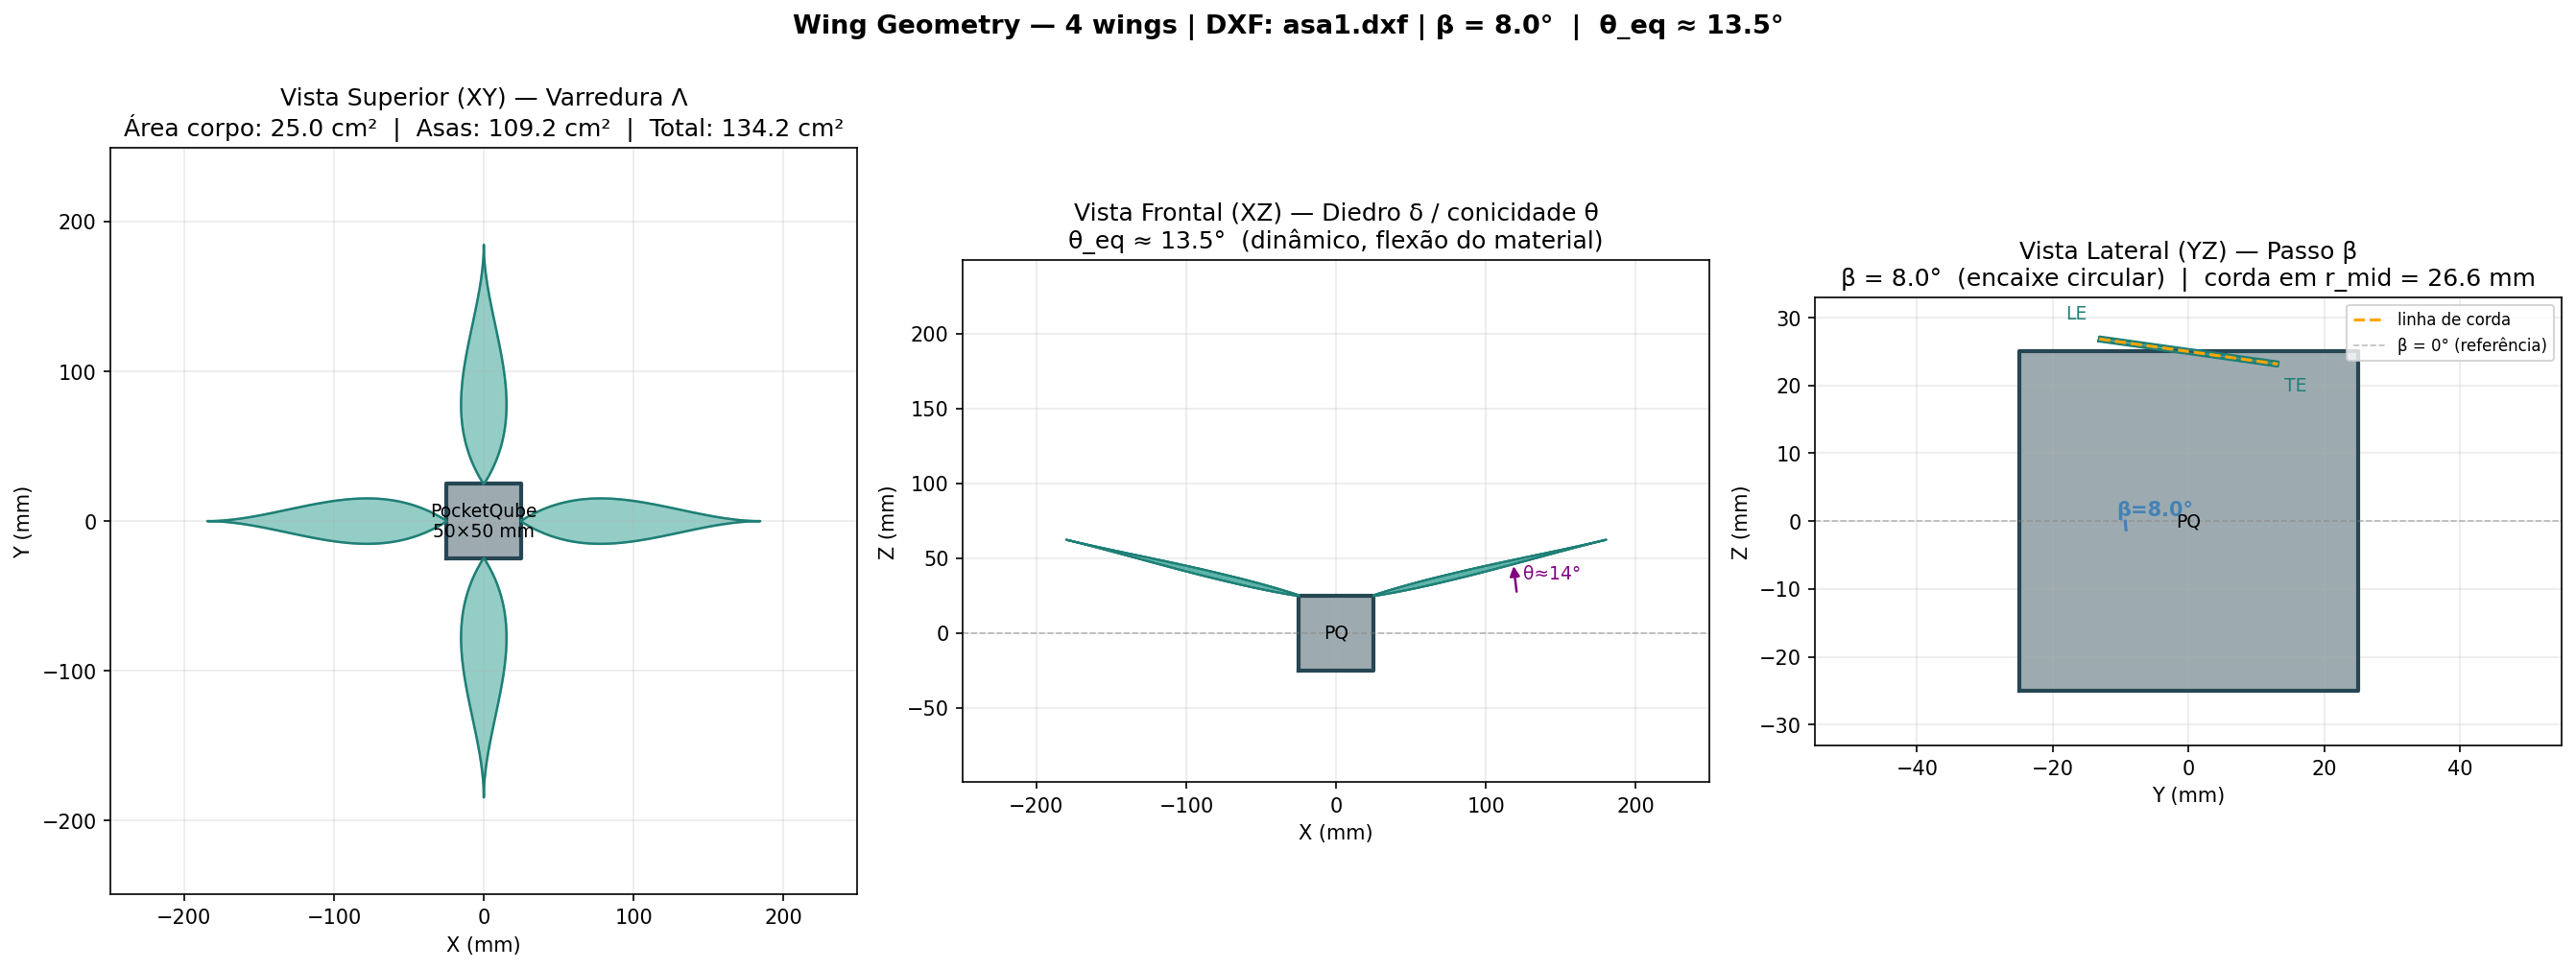
\includegraphics[width=0.85\textwidth]{fig_test1_geom.png}
\caption{Vistas geométricas do Teste 1 (Asa1).}
{\footnotesize\centering Fonte: Autores (2026)\par}
\label{fig:test1_geom}
\end{figure}

\begin{figure}[htbp]
\centering

\includegraphics[width=0.85\textwidth]{fig_test2_lrr.png}
\caption{LRR do Teste 2 (Asa2, 4 asas, 200~g).}
{\footnotesize\centering Fonte: Autores (2026)\par}
\label{fig:test2_lrr}
\end{figure}

\begin{figure}[htbp]
\centering
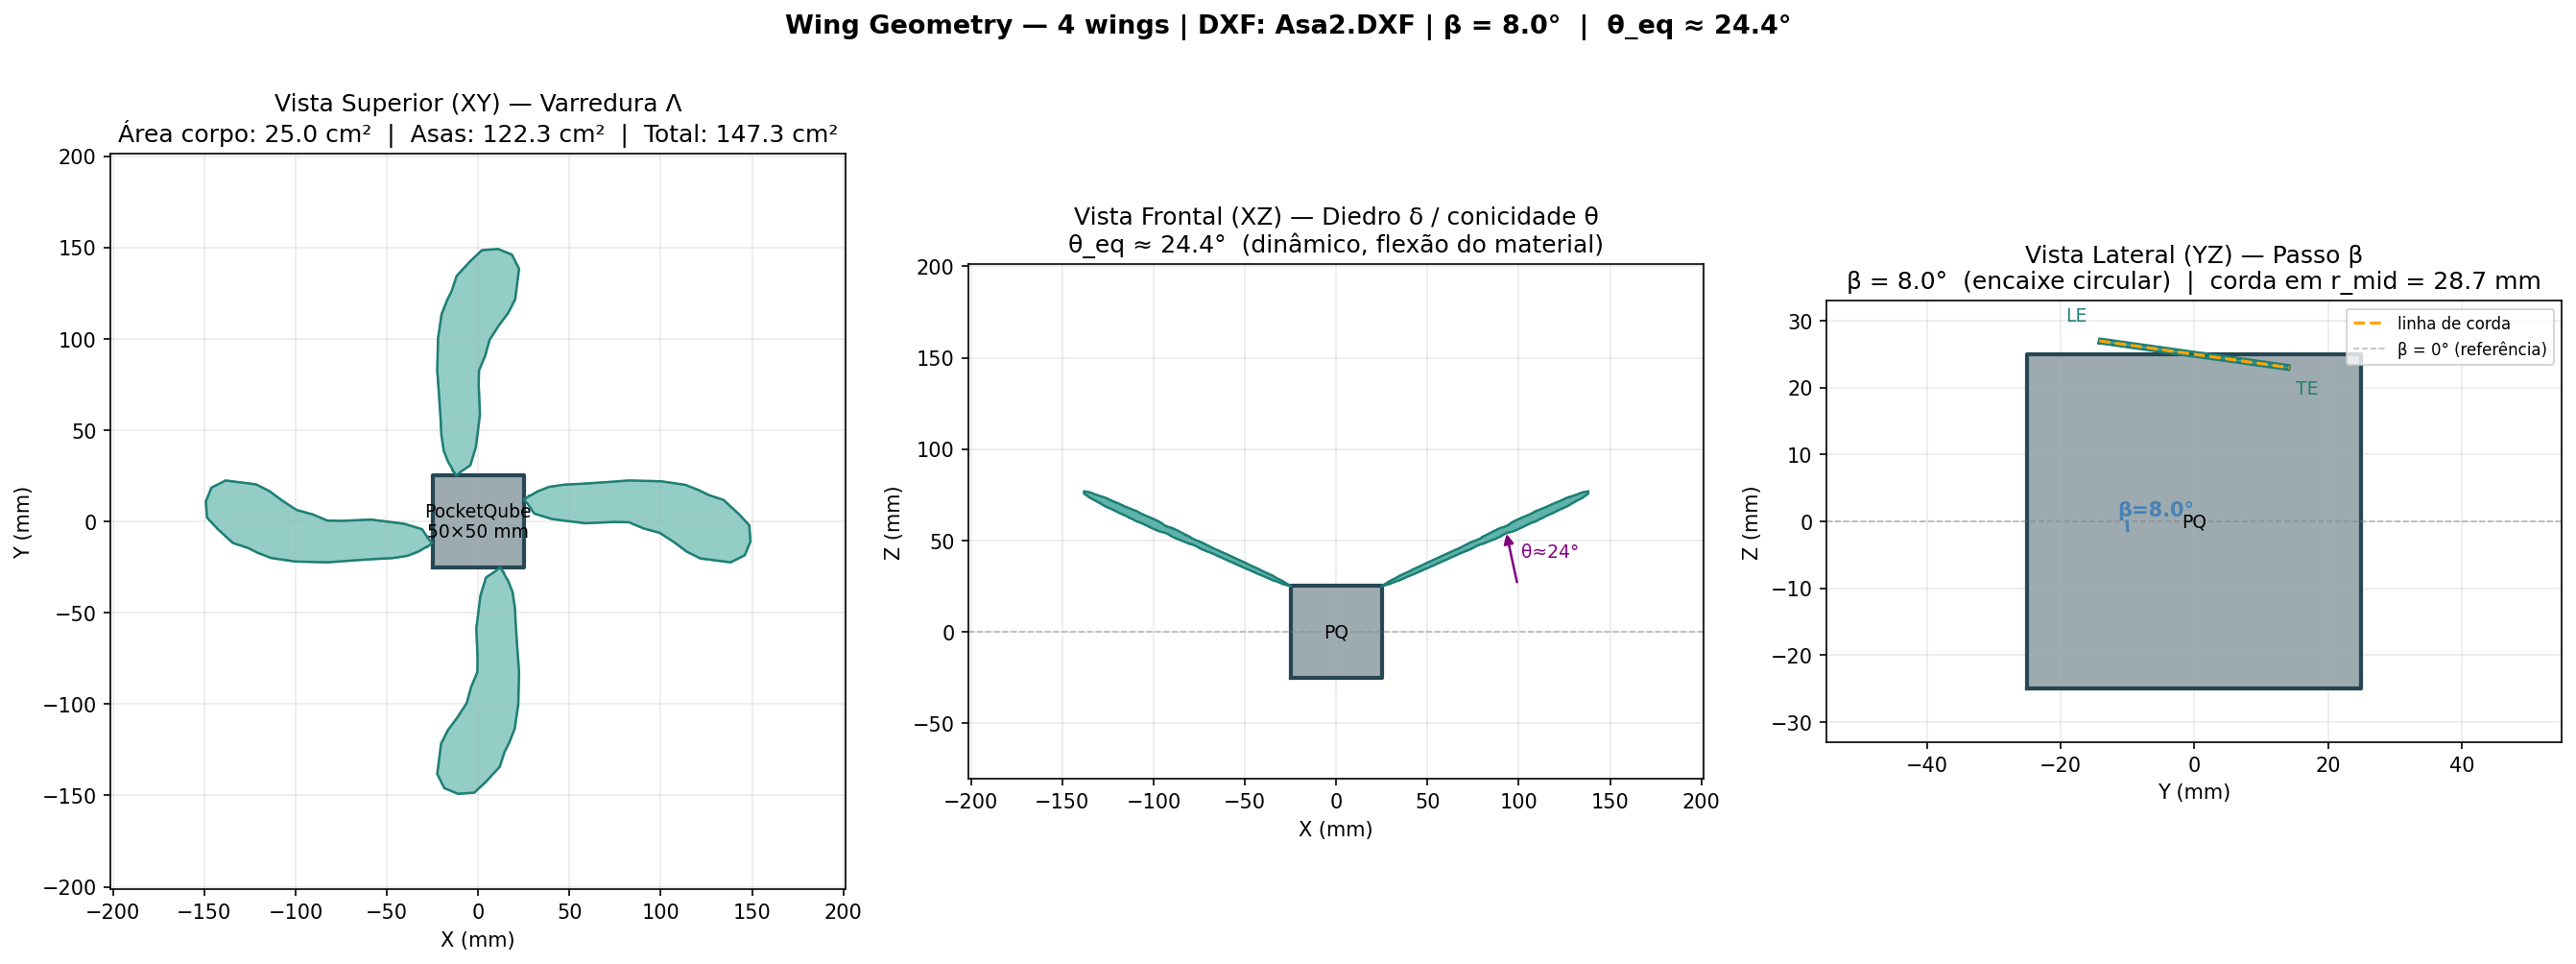
\includegraphics[width=0.85\textwidth]{fig_test2_geom.png}
\caption{Vistas geométricas do Teste 2 (Asa2).}
{\footnotesize\centering Fonte: Autores (2026)\par}
\label{fig:test2_geom}
\end{figure}

\subsection{Simulação computacional da configuração Asa3 com 4 asas (Teste 3)}

A Tabela~\ref{tab:test3} apresenta os resultados da simulação da configuração Asa3.DXF com 4 asas em altitude operacional de 1000~m.

\begin{table}[htbp]
\caption{Resultados da simulação computacional para o Teste 3 (Asa3, 4 asas).}
\centering
\begin{tabular*}{\textwidth}{@{\extracolsep{\fill}}lc}
\hline
Parâmetro & Valor \\
\hline
Geometria & Asa3.DXF, 4 asas \\
Massa total [g] & 200 \\
Velocidade de impacto [m/s] & 12,90 \\
 Tempo de descida [s] & 78,03 \\
Conicidade $\theta$ de equilíbrio [$^\circ$] & 17,22 \\
Taxa de rotação [RPM] & 371,98 \\
Energia cinética final [J] & 16,65 \\
Energia potencial inicial [J] & 1962,00 \\
Energia dissipada [J] (\%) & 1945,35 (99,15\%) \\
\hline
\end{tabular*}
{\footnotesize\centering Fonte: Autores (2026)\par}
\label{tab:test3}
\end{table}

A configuração com 4 asas apresenta velocidade de impacto de 12,90~m/s, com conicidade de 17,22$^\circ$ e spin de 372~RPM, priorizando estabilidade cônica e margem de segurança na dissipação de energia.

\begin{figure}[htbp]
\centering
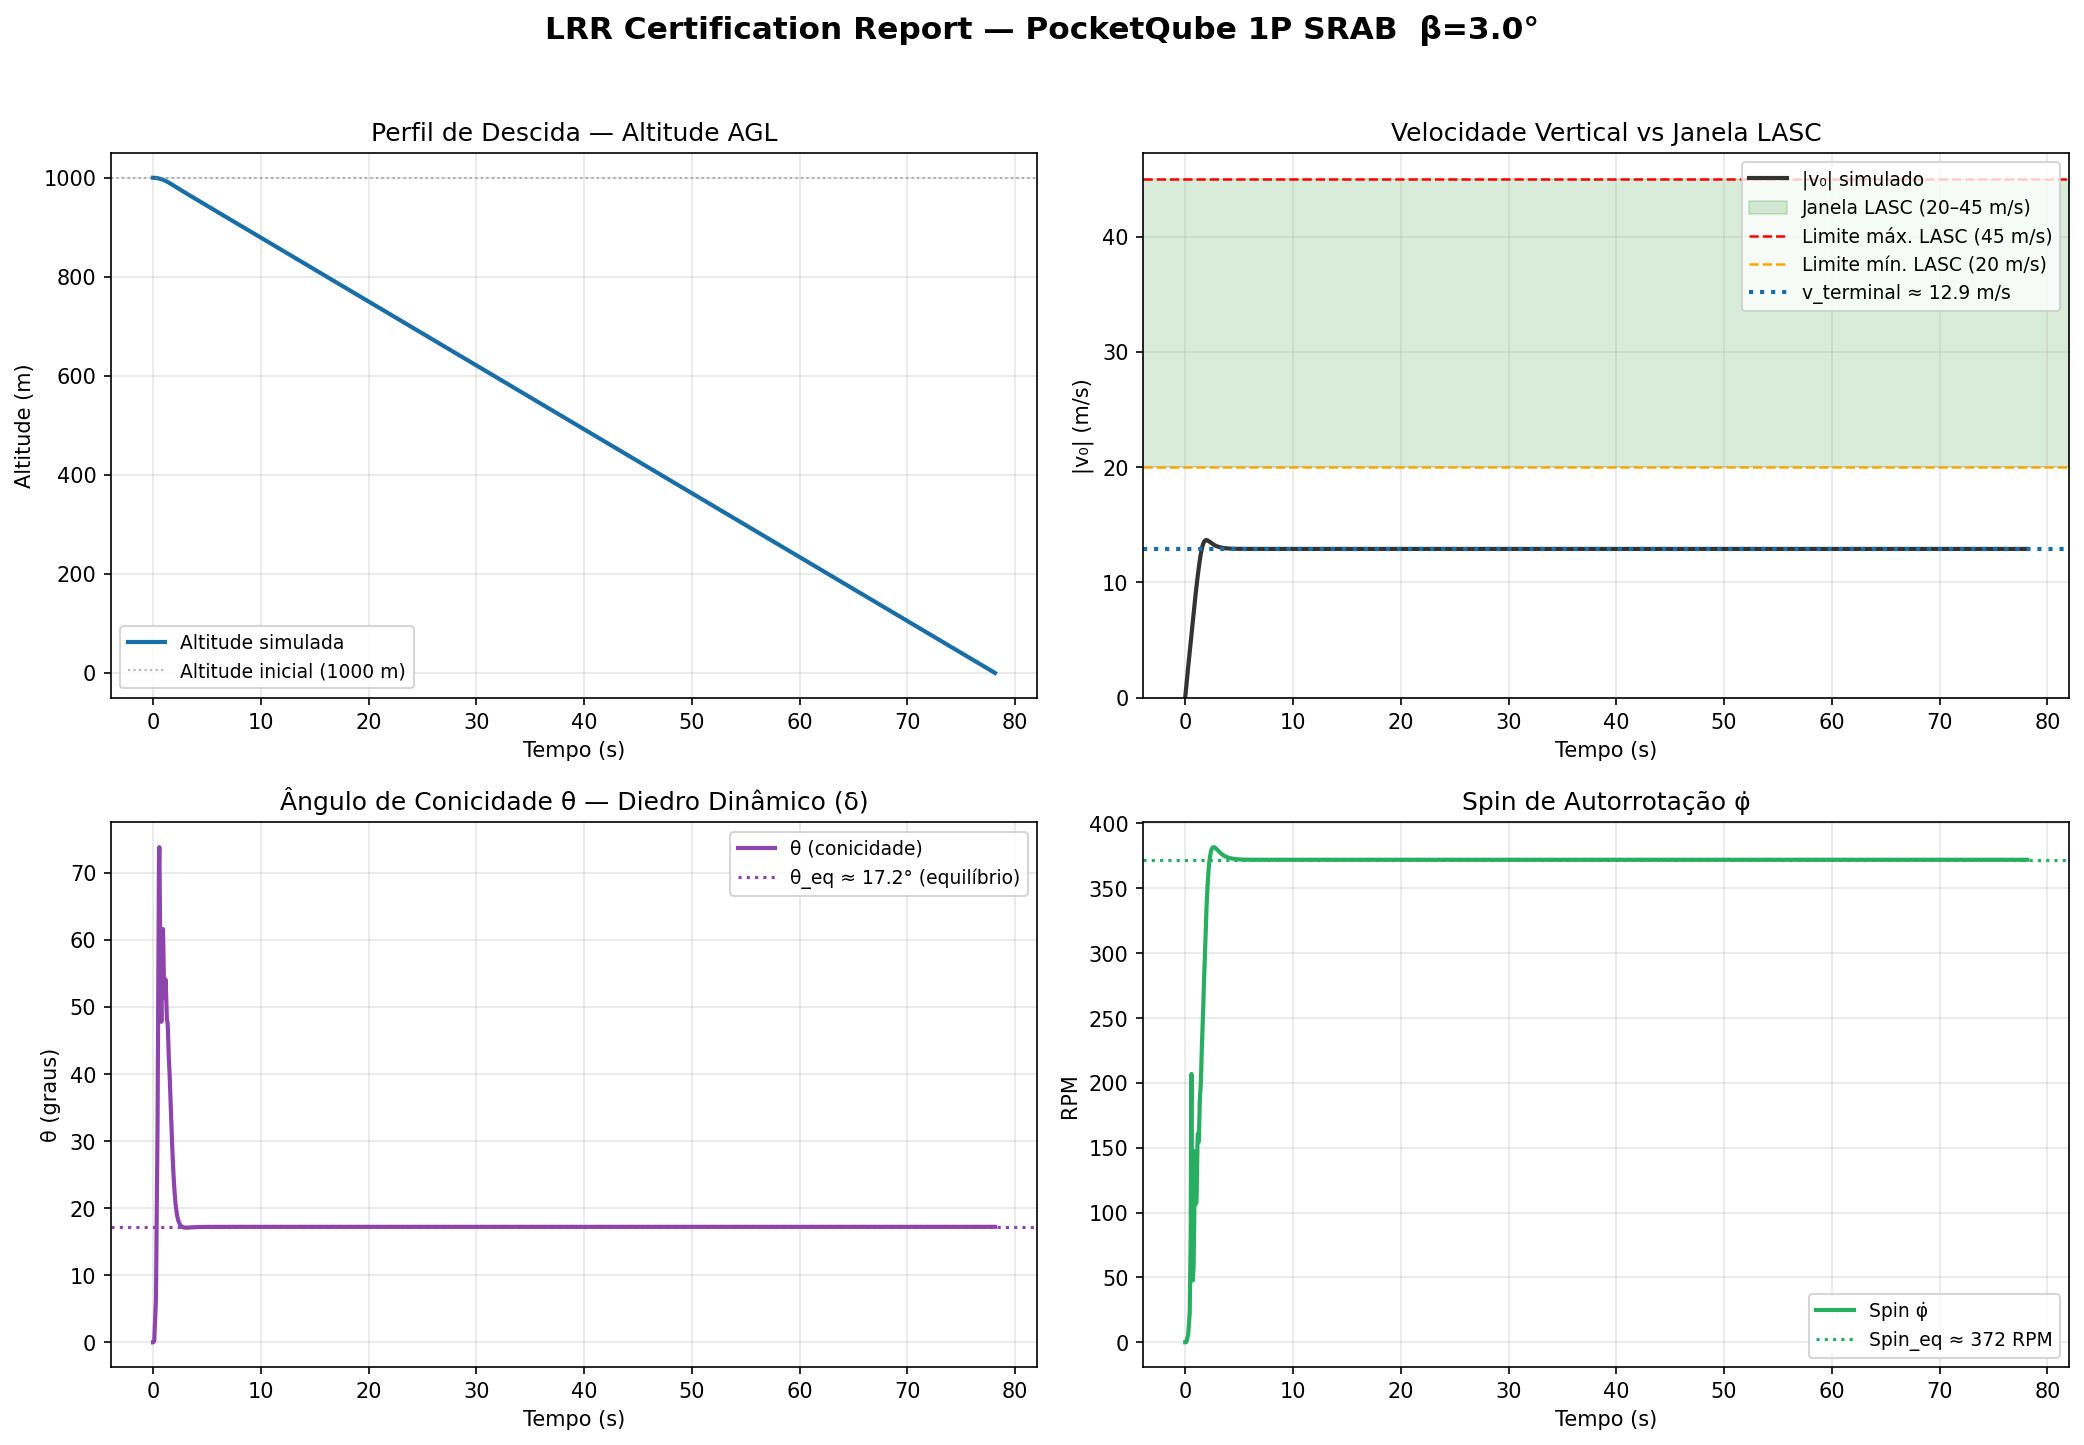
\includegraphics[width=0.85\textwidth]{fig_test3_lrr.png}
\caption{LRR do Teste 3 (Asa3, 4 asas, 200~g). Velocidade de impacto de 12,90~m/s com conicidade de 17,22$^\circ$.}
{\footnotesize\centering Fonte: Autores (2026)\par}
\label{fig:test3_lrr}
\end{figure}

\begin{figure}[htbp]
\centering
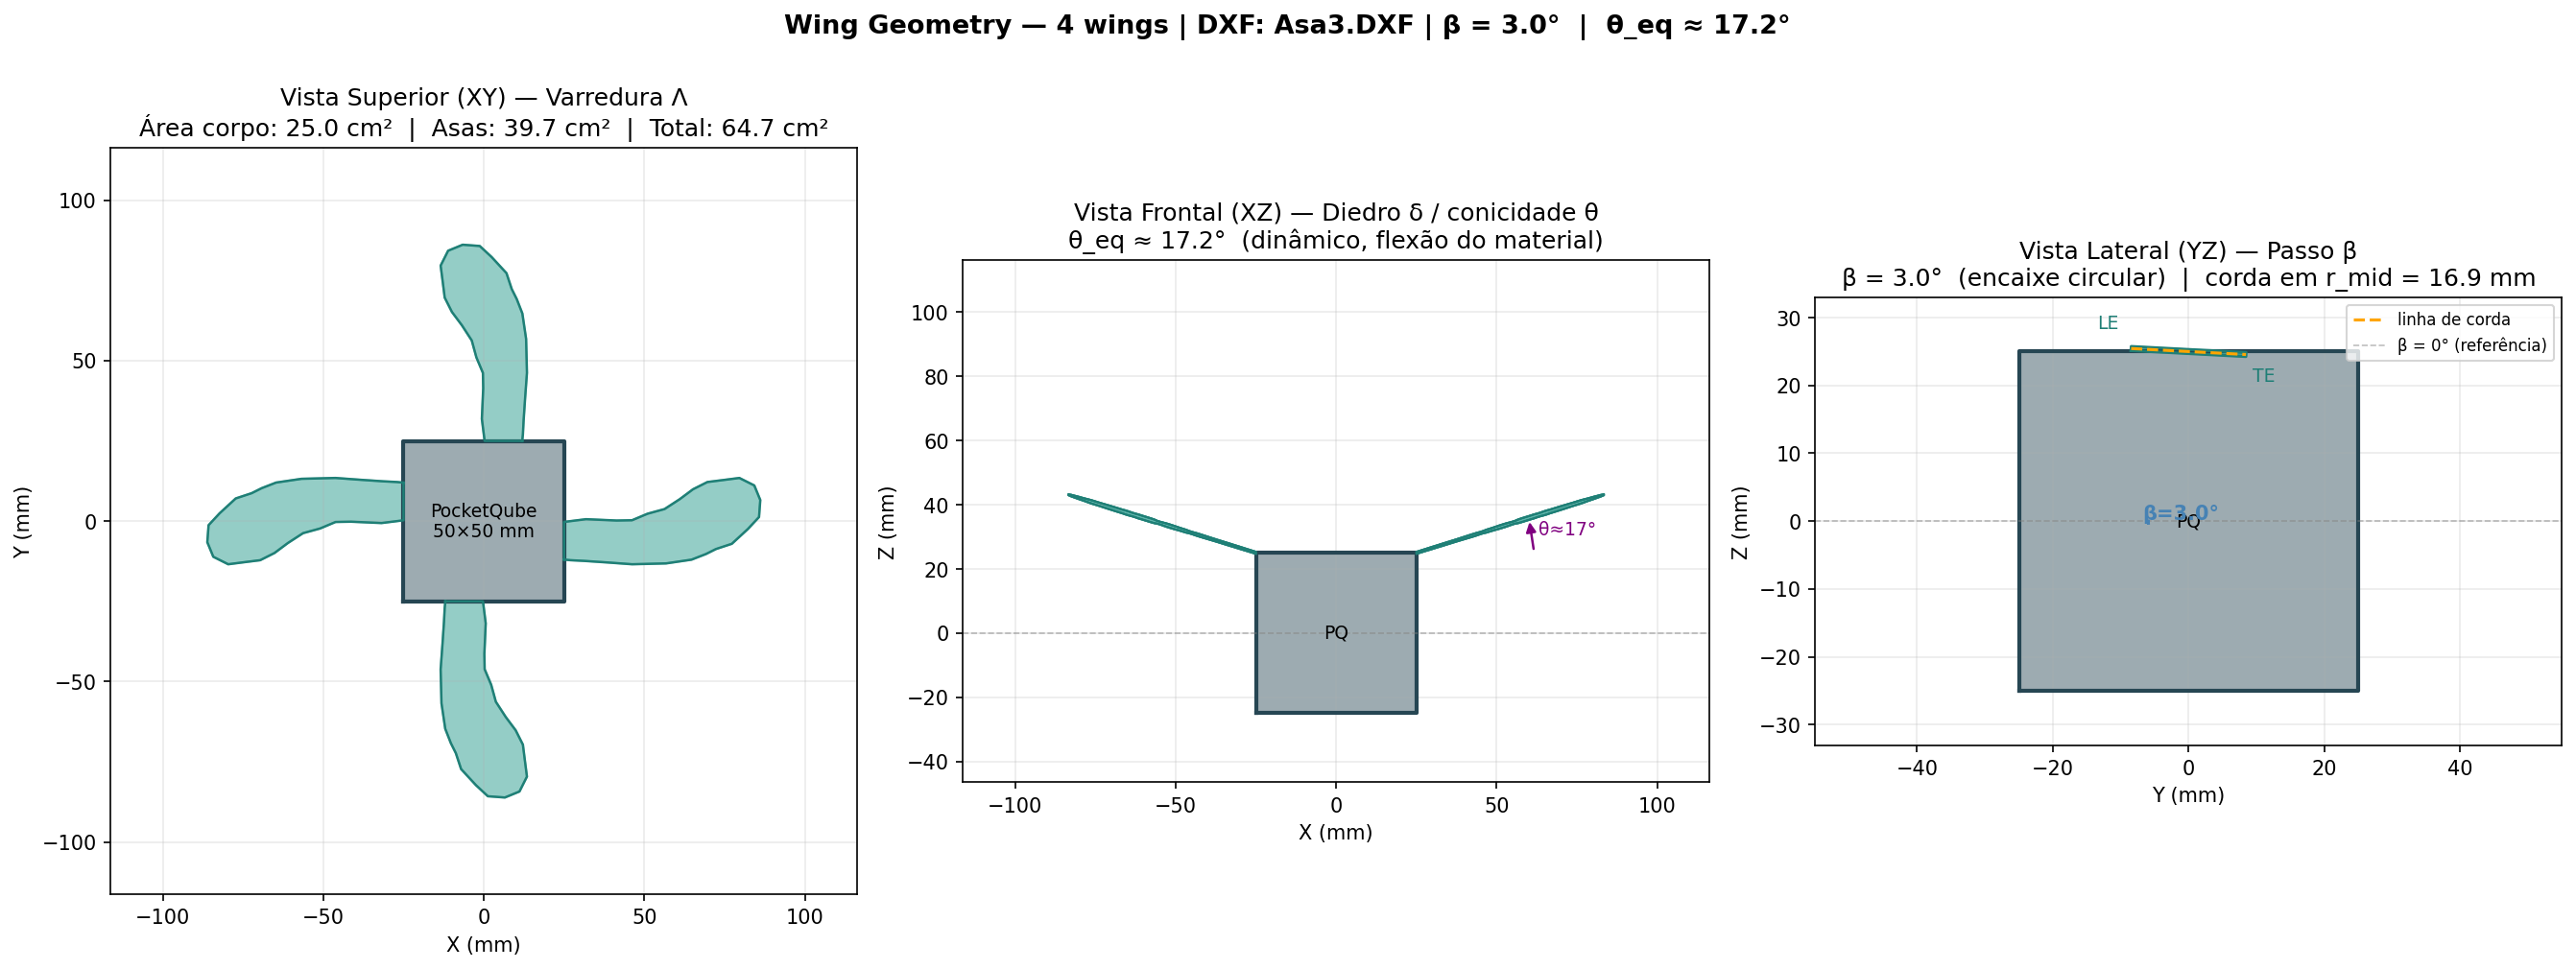
\includegraphics[width=0.85\textwidth]{fig_test3_geom.png}
\caption{Vistas geométricas do Teste 3 (Asa3, 4 asas).}
{\footnotesize\centering Fonte: Autores (2026)\par}
\label{fig:test3_geom}
\end{figure}

\subsubsection*{Análise de Sensibilidade Monte Carlo (Teste 3)}

Para quantificar a dispersão esperada, conduziu-se análise Monte Carlo com 200 iterações, variando simultaneamente a massa total (200~$\pm$~10~g), o ângulo de passo $\beta$ (3,0$^\circ$~$\pm$~0,5$^\circ$), $C_{D0}$ (1,0~$\pm$~0,10) e $f_{factor}$ (0,3~$\pm$~0,03). Os intervalos foram definidos com base nas tolerâncias de fabricação estimadas para impressão PETG a 0,6~mm ($\beta$ e $f_{factor}$), na faixa de calibração observada nos Testes 1 e 2 ($C_{D0}$) e na margem regulatória de massa do padrão PocketQube 1P. A Tabela~\ref{tab:mc} sumariza os resultados.

\begin{table}[htbp]
\caption{Resultados da análise Monte Carlo para a configuração Asa3 com 4 asas (200 iterações).}
\centering
\begin{tabular*}{\textwidth}{@{\extracolsep{\fill}}lccc}
\hline
Métrica & Média $\pm$ $\sigma$ & P5 & P95 \\
\hline
Velocidade de impacto & 12,89 $\pm$ 0,20~m/s & 12,54~m/s & 13,19~m/s \\
Tempo de descida & 78,23 $\pm$ 1,22~s & 76,46~s & 80,38~s \\
Conicidade $\theta_{eq}$ & 17,48$^\circ$ $\pm$ 1,19$^\circ$ & 15,71$^\circ$ & 19,50$^\circ$ \\
Spin de equilíbrio & 371 $\pm$ 8~RPM & 358~RPM & 384~RPM \\
Energia de impacto & 16,54 $\pm$ 1,19~J & 14,40~J & 18,30~J \\
\hline
\end{tabular*}
{\footnotesize\centering Fonte: Autores (2026)\par}
\label{tab:mc}
\end{table}

A velocidade de impacto apresenta baixa dispersão ($\sigma = 0,20$~m/s, CV~$<$~2\%). O P95~=~13,19~m/s é uma estimativa preliminar (200 iterações são suficientes para média e desvio; recomenda-se 1000 para quantis extremos), ainda abaixo do limite LASC de 45~m/s.

\subsection{Limitações e trabalhos futuros}

Os Testes 1 e 2 foram conduzidos em $\sim$20~m, insuficientes para regime terminal, e o modelo atmosférico é simplificado ($\rho$ constante), sem vento ou turbulência. Como trabalhos futuros, propõe-se:

\begin{enumerate}
  \item Teste 3 (campo): lançamento real com critérios de erro $< \pm 5\%$ em velocidade e $< \pm 3\%$ em tempo.
  \item Integração com RocketPy para perfil atmosférico variável (GFS/ISA), deriva por vento e visualização 3D \citep{rocketpy2024}.
  \item Recalibração de $C_{D0}$ e $f_{factor}$ pós-testes.
  \item Análise de sensibilidade expandida incluindo $f_{factor}$ e $\beta$.
\end{enumerate}

\subsection{Benchmark SRAB vs paraquedas}

Comparação entre SRAB (Asa3, 4 asas, 200~g) e paraquedas flat circular de $\varnothing$200~mm ($C_D = 1,5$) a partir de 1000~m (Tabela~\ref{tab:benchmark}).

\begin{table}[htbp]
\caption{Comparativo SRAB vs Paraquedas.}
\centering
\begin{tabular*}{\textwidth}{@{\extracolsep{\fill}}lcc}
\hline
Parâmetro & SRAB (4 asas) & Paraquedas ($\varnothing$200~mm) \\
\hline
Massa total [g] & 200 & 200 \\
Velocidade de impacto [m/s] & 12,90 & 8,25 \\
Tempo de descida [s] & 78,03 & 118,33 \\
Energia de impacto [J] & 16,65 & 6,80 \\
Abaixo do limite LASC (45~m/s) & Sim & Sim \\
Dentro da janela LASC (20--45~m/s) & Não & Não \\
\hline
\end{tabular*}
{\footnotesize\centering Fonte: Autores (2026)\par}
\label{tab:benchmark}
\end{table}

O SRAB atinge 1,6$\times$ a velocidade do paraquedas, porém elimina pontos únicos de falha (acionamento, linhas, costuras) e reduz o tempo de descida em 34\%, diminuindo a deriva por vento.

%%%%%%%%%%%%%%%%%%%%%%%%%%%%%%%%%%%%%%%%%%%%%%%%%%%%%%%%%%%%%%%%%%%%%%
% 6. CONCLUSÕES
%%%%%%%%%%%%%%%%%%%%%%%%%%%%%%%%%%%%%%%%%%%%%%%%%%%%%%%%%%%%%%%%%%%%%%

\section{CONCLUSÕES}

Este trabalho apresentou o desenvolvimento e a validação preliminar do SRAB para PocketQube 1P, com cinco contribuições principais alinhadas aos objetivos propostos: (a) o modelo dinâmico de 4$^{\underline{a}}$ ordem acoplado ao BEM foi validado qualitativamente nos Testes 1 e 2, com a transição Asa1--Asa2 resultando em aumento de 81,6\% na conicidade de impacto (de 13,46$^\circ$ para 24,44$^\circ$), consistente com a melhoria qualitativa observada em campo; (b) a instrumentação embarcada (ESP32-C3, ICM-20602, BMP280, LoRa RFM95W) foi validada funcionalmente em bancada a 20~Hz, com detecção de apogeu e logging em LittleFS sem perda de amostras; (c) a simulação da configuração Asa3 com 4 asas em altitude operacional de 1000~m resultou em velocidade de impacto de 12,90~m/s, conicidade de equilíbrio de 17,22$^\circ$ e spin de 372~RPM, com dissipação de 99,15\% da energia potencial inicial; (d) a análise de sensibilidade demonstrou que a velocidade terminal é independente de $C_{D0}$ na faixa de $\pm20\%$, confirmando que a sustentação aerodinâmica e não o arrasto basal é o mecanismo dominante no regime de autorrotação estável; (e) o benchmark com paraquedas flat circular de 200~mm mostrou que o SRAB atinge 1,6$\times$ a velocidade de impacto (12,90~m/s contra 8,25~m/s) com tempo de descida 34\% menor (78,03~s contra 118,33~s), eliminando pontos únicos de falha associados a mecanismos de acionamento, linhas e costuras.

A análise Monte Carlo (200 iterações) indicou velocidade de impacto de 12,89~$\pm$~0,20~m/s (P95~=~13,19~m/s, CV~$<$~2\%), confirmando a robustez do sistema às variações paramétricas de massa, $\beta$, $C_{D0}$ e $f_{factor}$. A baixa dispersão observada decorre do regime de autorrotação estável, onde a velocidade terminal é determinada principalmente pela geometria das asas e pela massa total, com influência secundária dos parâmetros fenomenológicos calibrados. Ambas as configurações simuladas operam abaixo da janela regulatória LASC (20--45~m/s), indicando que ajustes geométricos adicionais como redução do número de asas ou aumento do ângulo de passo $\beta$ são necessários para conformidade regulatória.

O SRAB demonstra viabilidade como sistema passivo de recuperação para PocketQubes, oferecendo vantagens de confiabilidade sobre paraquedas ao eliminar mecanismos de acionamento e pontos únicos de falha.

%%%%%%%%%%%%%%%%%%%%%%%%%%%%%%%%%%%%%%%%%%%%%%%%%%%%%%%%%%%%%%%%%%%%%%
% AGRADECIMENTOS
%%%%%%%%%%%%%%%%%%%%%%%%%%%%%%%%%%%%%%%%%%%%%%%%%%%%%%%%%%%%%%%%%%%%%%

\subsection*{\textit{Agradecimentos}}

Os autores agradecem à equipe Serra Rocketry (Missão Helike \#213), à Alba Orbital pela doação da plataforma PocketQube 1P e aos laboratórios do IPRJ/UERJ pelo suporte institucional.

%%%%%%%%%%%%%%%%%%%%%%%%%%%%%%%%%%%%%%%%%%%%%%%%%%%%%%%%%%%%%%%%%%%%%%
% REFERÊNCIAS
%%%%%%%%%%%%%%%%%%%%%%%%%%%%%%%%%%%%%%%%%%%%%%%%%%%%%%%%%%%%%%%%%%%%%%

\bibliographystyle{apalike}
\fontsize{11}{0}\selectfont
\bibliography{bib/references}

%%%%%%%%%%%%%%%%%%%%%%%%%%%%%%%%%%%%%%%%%%%%%%%%%%%%%%%%%%%%%%%%%%%%%%
% TRADUÇÃO PARA INGLÊS (EXIGÊNCIA DO TEMPLATE)
%%%%%%%%%%%%%%%%%%%%%%%%%%%%%%%%%%%%%%%%%%%%%%%%%%%%%%%%%%%%%%%%%%%%%%

\vspace{0.5cm}

\selectlanguage{english}

\vspace{0.2cm}

\noindent {\bfseries BIOINSPIRED AUTOROTATIVE RECOVERY SYSTEM (SRAB) FOR POCKETQUBE 1P NANOSATELLITE: FOUNDATIONS, MODELING, PRELIMINARY EXPERIMENTAL VALIDATION AND COMPUTATIONAL SIMULATION}

\vspace{0.5cm}

\begin{abstract}
The recovery of PocketQube 1P nanosatellites traditionally relies on parachutes, which present single points of failure such as folding errors, stitching defects or corrosion. This work proposes the Bioinspired Autorotative Recovery System (SRAB), based on the passive autorotation mechanism observed in samara seeds (\textit{Acer rubrum}, \textit{Fraxinus}). The system employs an asymmetric structural architecture that induces conical rotation without active actuation, generating a Leading-Edge Vortex (LEV) that reduces terminal velocity. Validation uses a fourth-order dynamic model (reduced Newton-Euler) coupled with Blade Element Theory (BEM), implemented in the Samara PQ simulator in Python, and qualitative free-fall experiments with two iterative prototypes (Tests 1 and 2). Computational simulation of the Asa3.DXF configuration with 4 wings (Test 3 -- Part A) resulted in impact velocity of 12.90~m/s, equilibrium conicity of 17.22$^\circ$ and spin of 372~RPM. Monte Carlo dispersion analysis (200 iterations) indicated impact velocity of 12.89~$\pm$~0.20~m/s (P95~=~13.19~m/s). The embedded instrumentation (ESP32-C3, ICM-20602, BMP280, LoRa RFM95W) was functionally validated at 20~Hz.
\end{abstract}

\noindent {\em Keywords: Passive recovery, samara, PocketQube, autorotation, Monte Carlo}

\selectlanguage{brazil}

\end{document}
